\documentclass[a4paper,english]{article}
\usepackage{graphicx}
\usepackage{listings}
%% Use utf-8 encoding for foreign characters
%%\usepackage[T1]{fontenc}
%%\usepackage[utf8]{inputenc}
%%\usepackage{babel}
%%
%%%% Vector based fonts instead of bitmaps
%%\usepackage{lmodern}
%%
%%%% Useful
%%%\usepackage{fullpage} % Smaller margins
%%\usepackage{enumerate}
%%
%%%% Theorem
%%\usepackage{amsthm}
%%
%%%% More math
%%\usepackage{amsmath}
%%\usepackage{amssymb}

%% Document Header
\title{Section3}
\author{Elliott Ashby}
\date{\today}

\begin{document}
    \maketitle
    \section{q1}
    \lstinputlisting[language=Python, firstline=4, lastline=5]{./q4_1.py} 
        This is a function that returns the result of the integrand.
        We can then input it into trap0 like:
    \lstinputlisting[language=Python, firstline=39, lastline=43]{./q4_1.py}
        Here, if the change in the returned value is smaller than $1.0e^{-6}$ the list stops
        being added to as n increases, meaning a[-1] is the final value with an accuracy
        of $1.0e^{-6}$.
        \\
    \section{q2}
        Printing a[-1] and n after running the above code results in
        \begin{center}
            $\int_0^1{\frac{x^4(1-x)^4}{1+x^2}dx} = 0.0012649570769764054$
        \end{center}
        \\
    \section{q3}
        This result in section q2 results from 7 trapeziums.
        \\
    \section{q4}
        Using:
        \lstinputlisting[language=Python]{./q4_4.py}
        We print a value for the integral
        \begin{center}
            $\int_{-\infty}^\infty{e^{-x^2}dx} = 1.7724538509055157$
        \end{center}
        \\
    \section{q5}
    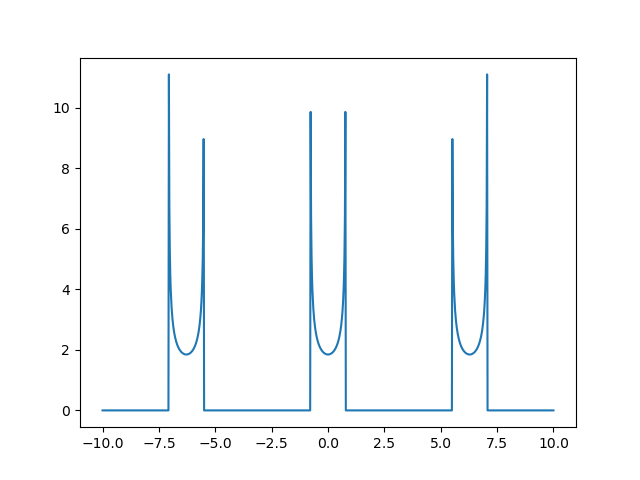
\includegraphics[scale=0.8]{./q4_5.png}
        Here, we can see spikes to infinity at values where $\alpha = \theta$. The inconsistent height
        of the asymptotes are because only 1000 discrete value were calculated to graph, meaning that
        these asymptotes are only at $\alpha \approx \theta$.
        \\
    \section{q6}
        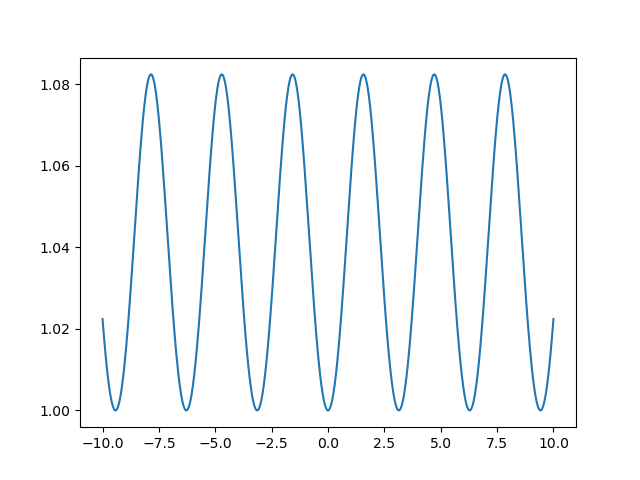
\includegraphics[scale=0.8]{./q4_6.png}
        Any numerical integration will fail due to division by zero.
        \\
        After changing the variable we plot as above.
        \\
    \section{q7}
    \lstinputlisting[language=Python, firstline=0, lastline=25]{./q4_7.py}
    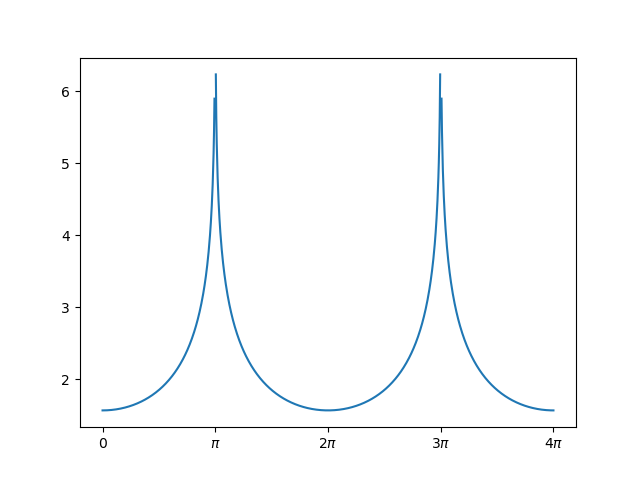
\includegraphics[scale=0.8]{q4_7.png}
        In this script we create a large list of 1000 numbers equally spaced 0 through $4\pi$.
        Then for each value of alpha we calculate the integral and add it to the end of a list.
        We can now tabulate the data since the appended list is a list of lists including the 
        alpha value used.
        \\
        Plotting the alpha vs the integral reveals that when alpha equals $\pi$ and $3\pi$ the integral
        is equal to infinity since this is also division by zero.
        \\
    \section{q8}
    \lstinputlisting[language=Python, firstline=27, lastline=36]{./q4_7.py}
        In order to gain a value of $T/T_0$ at $90^\circ$ we simply round both $\pi/2$ and 
        our values of alpha to 2 decimal places, find the index of where $\alpha \approx \pi/2$
        and print the associated ratio.
        \\
        \\
        at $\alpha = 90^\circ$:
    \begin{equation}
        \frac{T}{T_0} = \frac{2}{\pi}\int_0^{\pi/2}\frac{d\phi}{(1-\sin^2(\alpha/2)\sin^2\phi)^{1/2}} 
        = 1.1807649945835401
    \end{equation}
        \\
    \section{bonus}
    \lstinputlisting[language=Python]{./q4_bonus.py}
    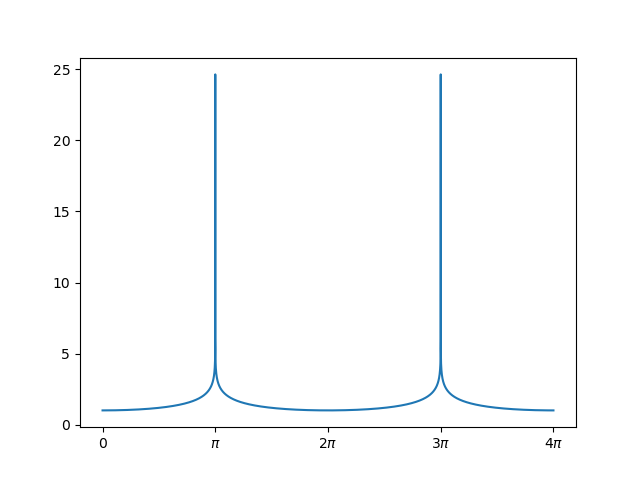
\includegraphics[scale=0.8]{./q4_bonus.png}
    Using the sympy package we can evaluate the integral in q6 entirely algebraicly and 
    then after doing so, sub in values for i$\alpha$, including subbing in specific values,
    either by subbing in separetely or inserting specific values into the list created 
    in order to graph $\alpha$ vs $T/T_0$.
    \\
    \\
    Subbing $\pi/2$ directly into $\alpha$ of the integrated equation and multiplying by $2/\pi$ 
    gives a result:
    \begin{equation}
        \frac{T}{T_0} = \frac{2}{\pi}\int_0^{\pi/2}\frac{d\phi}{(1-\sin^2(\alpha/2)\sin^2\phi)^{1/2}} 
        = 1.18034059901610
    \end{equation}
\end{document}
